\documentclass[compress]{beamer}
%\documentclass[ignorenonframetext,handout]{beamer}
%\setbeamercovered{transparent}
%\usepackage[ISO 8859-1]{inputenc}
\usepackage{default}

% para usar figuras devemos acrescentar
\usepackage{graphicx}
%\usepackage{graphics}
%\DeclareGraphicsExtensions{.pdf,.png,.jpg}
%\DeclareGraphicsExtensions{.jpg, .eps}
%\DeclareGraphicsRule{.jpg}{eps}{.jpg}{`jpeg2ps -h -r 600 #1}
\usepackage{tikz}
%\usetikzlibrary{arrows,backgrounds,coordinatesystems,3d,shapes,plotmarks,automata,calendar,er,
%folding,matrix,mindmap,patterns,petri,plothandlers,topaths,trees} 
\usetikzlibrary{positioning}
%\usepgflibrary{decorations.pathreplacing}
\usetikzlibrary{decorations.pathreplacing}
\usetikzlibrary{decorations.pathmorphing}
\usetikzlibrary[patterns]
%\tikzstyle{every text node part}
%\usetikzlibrary{arrows,backgrounds,positioning,fit} 
\usetikzlibrary{calc}
% para gerar graficos no latex
\usepackage{pgfplots}
\pgfplotsset{compat=newest}

% Include the listings-package
\usepackage{listings}    
\usepackage{epigraph}

\usepackage{amsfonts}
\usepackage{amssymb}
\usepackage{amsmath}
\usepackage{MnSymbol}

\usepackage[brazil]{babel}
\usepackage[utf8]{inputenc}

% \usepackage{algpseudocode}
% \usepackage{algorithmicx}
\usepackage[Algoritmo]{algorithm}
\usepackage[noend]{algorithmic}

\usepackage[author={Max Schlepzig}]{pdfcomment}

\setbeamertemplate{bibliography entry title}{}
\setbeamertemplate{bibliography entry location}{}
\setbeamertemplate{bibliography entry note}{}

\newcounter{saveenumi}
\newcommand{\seti}{\setcounter{saveenumi}{\value{enumi}}}
\newcommand{\conti}{\setcounter{enumi}{\value{saveenumi}}}

%\usepackage{shadethm}

%\definecolor{shadethmcolor}{rgb}{.75,.75,.75}

%\newshadetheorem{theorem}{\scshape Teorema}[chapter]
\newtheorem{teorema}[theorem]{\scshape Teorema}
\newtheorem{proposicao}[theorem]{\scshape Proposição}
\newtheorem{corolario}[theorem]{\scshape Corolário}
\newtheorem{lema}[theorem]{\scshape Lema}
\newtheorem{definicao}[theorem]{\scshape Definição}
\newtheorem{conjectura}[theorem]{\scshape Conjectura}
\newtheorem{escolio}[theorem]{\scshape Escólio}
\newtheorem{exemplo}[theorem]{\scshape Exemplo}
\newtheorem{exemplos}[theorem]{\scshape Exemplos}
\newtheorem{propriedade}[theorem]{\scshape Propriedade}

\renewcommand{\u}{{\bf u}}
\renewcommand{\v}{{\bf v}}
\renewcommand{\sin}{\operatorname{sen}}
\renewcommand{\tan}{\operatorname{tg}}
\providecommand{\cas}{\operatorname{cas}}
\providecommand{\mdc}{\mathrm{mdc}}
\providecommand{\f}{{\bf f}}

\newcommand{\ie}{\textit{i.e.}}
\newcommand{\eg}{\textit{e.g.}}
%\newcommand{\qed}{\hfill $\square$}

\renewcommand\Re{\operatorname{Re}}
\renewcommand\Im{\operatorname{Im}}

\providecommand{\x}{{\bf x}}
\providecommand{\y}{{\bf y}}
\providecommand{\w}{{\bf w}}
\providecommand{\f}{{\bf f}}
\providecommand{\q}{{\bf q}}
\providecommand{\bfa}{{\bf a}}
\providecommand{\bfb}{{\bf b}}
\providecommand{\bfc}{{\bf c}}
\providecommand{\bfd}{{\bf d}}
\providecommand{\bfe}{{\bf e}}
\providecommand{\bfs}{{\bf s}}
\providecommand{\bfz}{{\bf z}}
\providecommand{\zero}{{\bf 0}}
\providecommand{\spn}{\mathrm{span}}
\providecommand{\posto}{\mathrm{posto}}
\providecommand{\nul}{\mathrm{nul}}
\providecommand{\proj}{\mathrm{proj}}
\providecommand{\tr}{\mathrm{tr}}
\providecommand{\sgn}{\mathrm{sgn}}

\providecommand{\cov}{\mathrm{cov}}

\providecommand{\dilation}{\mathcal{D}}
\providecommand{\erosion}{\mathcal{E}}
\providecommand{\open}{\mathcal{O}}
\providecommand{\close}{\mathcal{C}}

\newcommand*{\Bhat}{\skew{3}{\hat}{B}}

\setlength{\abovecaptionskip}{1px}
\setbeamertemplate{caption}{\raggedright\insertcaption\par}

\mode<presentation>
{
  \setbeamertemplate{background canvas}[vertical shading][bottom=white!10,top=blue!10]
%  \usetheme{Berkeley}
%  \usetheme{CambridgeUS}
%  \usetheme{Madrid}
  \usetheme{Warsaw}
  \usefonttheme[onlysmall]{structurebold}
  
  \setbeamertemplate{headline}{}
  
%   \setbeamercovered{invisible} % default
  \setbeamercovered{ transparent, again covered={\opaqueness{25}} } % =15%
%   \setbeamercovered{transparent=50}
%   \setbeamercovered{dynamic}

%   \setbeamercovered{again covered={\opaqueness<1->{25}}}
}

% copiado do site:
% http://latex-beamer-class.10966.n7.nabble.com/Covering-images-transparent-i-e-dimmed-figures-td1504
% . html
\usepackage{ifthen}

\usepackage{xcolor}


\makeatletter
\newcommand{\includecoveredgraphics}[2][]{
    \ifthenelse{\the\beamer@coveringdepth=1}{
        \tikz
            \node[inner sep=0pt,outer sep=0pt,opacity=0.15]
                {\includegraphics[#1]{#2}};
    }{
        \tikz
            \node[inner sep=0pt,outer sep=0pt]
                {\includegraphics[#1]{#2}};%
    }
}
\makeatother % não sei se precisa...

%\pgfdeclareimage[height=1.4cm]{logo_XIVsm}{semanauniversitaria}

%% put XIVsm logo in bottom left
%\setbeamertemplate{sidebar left}{
%%   \vfill%
 %  \rlap{\hskip0.0cm
  %       %\href{http://www.uece.br/semanauniversitaria}
   %      {\pgfuseimage{logo_XIVsm}}}
   %%\vskip2pt%
   %%\llap{\usebeamertemplate***{navigation symbols}\hskip0.1cm}%
   %%\vskip2pt%
%}

% para a disciplina de Processamento de Imagens
\title{Objective-C vs. C++}
\subtitle{MAC5714 – Programação Orientada a Objetos}
\author{André M. Vale\\ \and  Evandro F. Giovanini}
\institute[USP] % (optional, but mostly needed)
{
  Departamento de Ciências da Computação\\
  Universidade de São Paulo
}
\date{19 de Maio de 2015}


\lstset{ %
  backgroundcolor=\color{white},   % choose the background color; you must add \usepackage{color} or \usepackage{xcolor}
  basicstyle=\footnotesize,        % the size of the fonts that are used for the code
  breakatwhitespace=false,         % sets if automatic breaks should only happen at whitespace
  breaklines=true,                 % sets automatic line breaking
  captionpos=b,                    % sets the caption-position to bottom
  commentstyle=\color{mygreen},    % comment style
  deletekeywords={...},            % if you want to delete keywords from the given language
  escapeinside={\%*}{*)},          % if you want to add LaTeX within your code
  extendedchars=true,              % lets you use non-ASCII characters; for 8-bits encodings only, does not work with UTF-8
  frame=single,                    % adds a frame around the code
  keepspaces=false,                 % keeps spaces in text, useful for keeping indentation of code (possibly needs columns=flexible)
  keywordstyle=\color{blue},       % keyword style
  language=C++,                 % the language of the code
  morekeywords={*,...},            % if you want to add more keywords to the set
  numbers=left,                    % where to put the line-numbers; possible values are (none, left, right)
  numbersep=5pt,                   % how far the line-numbers are from the code
  numberstyle=\tiny\color{mygray}, % the style that is used for the line-numbers
  rulecolor=\color{black},         % if not set, the frame-color may be changed on line-breaks within not-black text (e.g. comments (green here))
  showspaces=false,                % show spaces everywhere adding particular underscores; it overrides 'showstringspaces'
  showstringspaces=false,          % underline spaces within strings only
  showtabs=false,                  % show tabs within strings adding particular underscores
  stringstyle=\color{mymauve},     % string literal style
  tabsize=2,                       % sets default tabsize to 2 spaces
  title=\lstname                   % show the filename of files included with \lstinputlisting; also try caption instead of title
}


\begin{document}

\begin{frame}
  \titlepage
\end{frame}

\begin{frame}{Agenda}
  \begin{itemize}
  \item { Motivação }
  \item { Histórico }
  \item { Sintaxe }
  \begin{itemize}
    \item { Classes }
    \item { Métodos }
    \item { Objetos }
  \end{itemize}
  \item { Exemplos }
  \begin{itemize}
    \item { Herança }
    \item { Polimorfismo }
  \end{itemize}
  \item { Cenário Atual }
  \item { Conclusão }
  \end{itemize}
\end{frame}

\begin{frame}{Motivação}
  \begin{itemize}
  \item {
    Aparentemente a mesma ideia: C + Orientação a Objetos
  }
  \item {
    Filosofias diferentes
  }
  \end{itemize}
\end{frame}

\begin{frame}{Objective-C}{Histórico}
    \begin{columns}[T] % contents are top vertically aligned
    \begin{column}[T]{.8\textwidth} % each column can also be its own environment
        \begin{minipage}[c][.7\textheight][c]{\linewidth}
            \begin{itemize}
                \item {   
                  Motivação: reuso de código
                }
                % You can also specify when the content should appear
                % by using <n->:
                \item {
                  Inspirada em Smalltalk e C
                }
                \item {
                  1988: Sistema Operacional NeXTSTEP
                }
                % or you can use the \uncover command to reveal general
                % content (not just \items):
                \item {
                  1994: Padrão OpenStep
                }
                \item {
                  GNUstep - Implementação livre
                }
                \item {
                  1996: Apple adquire a NeXT e desenvolve o Mac OS X
                }
                \item {
                  2007: Apple lança o iPhone
                }
            \end{itemize}
        \end{minipage}
    \end{column}
    \begin{column}[T]{.2\textwidth} % alternative top-align that's better for graphics
        \begin{figure}
        \centering
        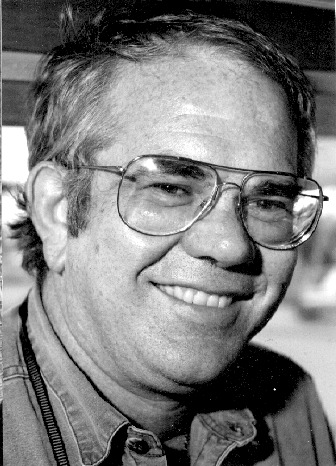
\includegraphics[width=2cm]{Brad.png}
        \caption{Brad Cox}
        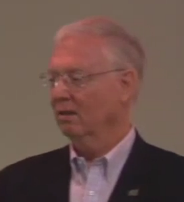
\includegraphics[width=2cm]{TomLove.png}
        \caption{Tom Love}
        \end{figure}
    \end{column}
    \end{columns}
\end{frame}

\begin{frame}{C++}{Histórico}
    \begin{columns}[T] % contents are top vertically aligned
    \begin{column}[T]{.8\textwidth} % each column can also be its own environment
        \begin{minipage}[c][.7\textheight][c]{\linewidth}
            \begin{itemize}
                \item {   
                    Motivação: adicionar funcionalidades a C
                }
                \item {   
                    1979: criada com o nome "C with Classes", influenciada por SIMULA.
                }
                \item {
                    1983: passou a ser C++, e logo depois foi publicado a referência The C++ Programming Language
                }
                \item {
                    1989: lançada a versão 2.0
                }
                \item {
                    1998: Padrão ISO C++98. Depois vieram C++11 e C++14.
                }
                \item {
                    Suporte no GCC em 1987. Visual C++ criado em 1993.
                }
            \end{itemize}
        \end{minipage}
    \end{column}
    \begin{column}[T]{.2\textwidth} % alternative top-align that's better for graphics
        \begin{figure}
        \centering
        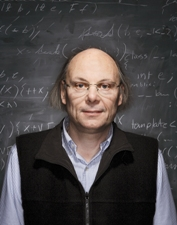
\includegraphics[width=2.5cm]{Bjarne.jpg}
        \caption{Stroustrup}
        \end{figure}
    \end{column}
    \end{columns}
\end{frame}

\begin{frame}{Classes - Objective C}
    \begingroup
        \ttfamily
        \lstinputlisting[firstline=7, lastline=19, firstnumber=7]{partida.m}
    \endgroup
\end{frame}

\begin{frame}{Métodos - Objective C}
    \begingroup
        \ttfamily
        \lstinputlisting[firstline=22, lastline=39, firstnumber=22]{partida.m}
    \endgroup
\end{frame}

\begin{frame}{Objetos - Objective C}
    \begingroup
        \ttfamily
        \lstinputlisting[firstline=44, lastline=52, firstnumber=44]{partida.m}
    \endgroup
\end{frame}

\begin{frame}{Classes - C++}
    \begingroup
        \ttfamily
        \lstinputlisting[firstline=7, lastline=16, firstnumber=7]{partida.cpp}
    \endgroup
\end{frame}

\begin{frame}{Métodos - C++}
    \begingroup
        \ttfamily
        \lstinputlisting[firstline=18, lastline=32, firstnumber=18]{partida.cpp}
    \endgroup
  
\end{frame}

\begin{frame}{Objetos - C++}
    \begingroup
        \ttfamily
        \lstinputlisting[firstline=36, lastline=40, firstnumber=36]{partida.cpp}
    \endgroup
\end{frame}

\begin{frame}{Exemplos}
    \begin{center}
    \huge{Vamos ver algo funcionando!}
    \end{center}
\end{frame}

\begin{frame}{Objective C - Cenário atual}
  \begin{figure}[h!]
    \centering
    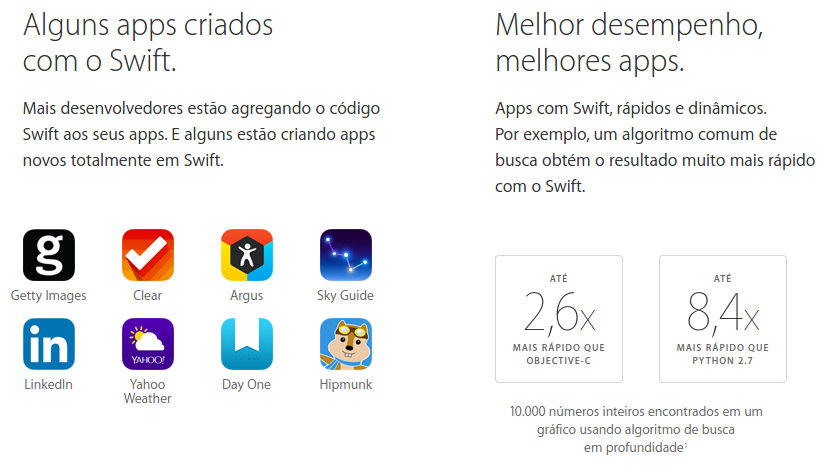
\includegraphics[width=1\textwidth]{Apple.png}
    \caption{\small \url{https://www.apple.com/br/swift/}}
    \caption{\small \url{https://developer.apple.com/}}
  \end{figure}
\end{frame}

\begin{frame}{C++ - Cenário atual}
  \setlength{\epigraphwidth}{0.9\textwidth}
  \renewcommand{\epigraphflush}{center}
  \epigraph{C makes it easy to shoot yourself in the foot;\\C++ makes it harder, but when you do it blows your whole leg off}{Bjarne Stroustrup}
\end{frame}

\begin{frame}{Utilização}
  \begin{figure}[h!]
    \centering
    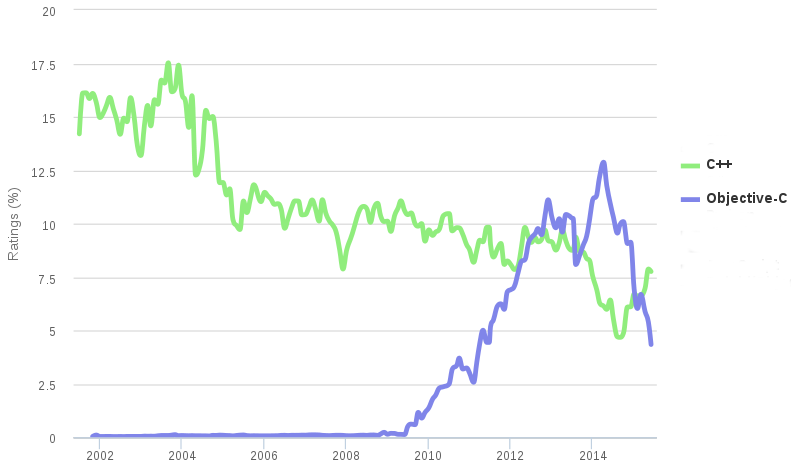
\includegraphics[width=1\textwidth]{Tiobe.png}
    \caption{\small \url{http://www.tiobe.com/}}
  \end{figure}
\end{frame}

\begin{frame}{Conclusão}
  \begin{itemize}
  \item {   
    C++ é mais similar a C que Objective-C.
  }
  \item {
    C++ foi desenvolvida na Bell Laboratories, o que pode ter colaborado para sua difusão.
  }
  \item {
    Desempenho (que foi o foco de Stroustrup).
  }
  \item {
    Vasta gama de ambientes de desenvolvimento para C++ enquanto Objective-C normalmente utiliza XCode.
  }
  \end{itemize}
\end{frame}

% All of the following is optional and typically not needed. 
\appendix
\section<presentation>*{\appendixname}
\subsection<presentation>*{Referências}

\begin{frame}[allowframebreaks]
  \frametitle<presentation>{Referências}
    
  \begin{thebibliography}{10}
    
  
  % Start with overview books.

  \beamertemplatebookbibitems
  \bibitem{Bjarne}
    STROUSTRUP,~Bjarne.
    \newblock {\em The C++ Programming Language.\\Addison-Wesley Professional, 4th edition, 2013.}
 
 \beamertemplatebookbibitems
  \bibitem{Aaron}
    HILLEGASS, Aaron e WARD, Mikey.
    \newblock {\em \\Objective-C Programming: The Big Nerd Ranch Guide.\\Big Nerd Ranch Guides, 2nd edition, 2013.}

  \setbeamertemplate{bibliography item}[online]
  \bibitem{Aaron}\url{https://developer.apple.com/}

  \setbeamertemplate{bibliography item}[online]
  \bibitem{Aaron}\url{http://www.w3schools.in/cplusplus/}
    
  \end{thebibliography}
\end{frame}

\end{document}